\documentclass[supercite]{Experimental_Report}
\title{~~~~~~~~~~~~}
\author{阮云轩}
%\coauthor{张三、李四}
\school{计算机科学与技术学院}
\classnum{CS2404}
\stunum{U202490035}
%\costunum{U202115631、U202115631}
\instructor{陈加忠} % 该系列实验报告模板由华科大计院教师陈加忠制作
\date{2024年11月22日}

\usepackage{algorithm, multirow}
\usepackage{algpseudocode}
\usepackage{amsmath}
\usepackage{amsthm}
\usepackage{framed}
\usepackage{mathtools}
\usepackage{subcaption}
\usepackage{xltxtra} %提供了针对XeTeX的改进并且加入了XeTeX的LOGO, 自动调用xunicode宏包(提供Unicode字符宏)
\usepackage{bm}
\usepackage{tikz}
\usepackage{tikzscale}
\usepackage{pgfplots}
%\usepackage{enumerate}

\pgfplotsset{compat=1.16}

\newcommand{\cfig}[3]{
	\begin{figure}[htb]
		\centering
		\includegraphics[width=#2\textwidth]{images/#1.tikz}
		\caption{#3}
		\label{fig:#1}
	\end{figure}
}

\newcommand{\sfig}[3]{
	\begin{subfigure}[b]{#2\textwidth}
		\includegraphics[width=\textwidth]{images/#1.tikz}
		\caption{#3}
		\label{fig:#1}
	\end{subfigure}
}

\newcommand{\xfig}[3]{
	\begin{figure}[htb]
		\centering
		#3
		\caption{#2}
		\label{fig:#1}
	\end{figure}
}

\newcommand{\rfig}[1]{\autoref{fig:#1}}
\newcommand{\ralg}[1]{\autoref{alg:#1}}
\newcommand{\rthm}[1]{\autoref{thm:#1}}
\newcommand{\rlem}[1]{\autoref{lem:#1}}
\newcommand{\reqn}[1]{\autoref{eqn:#1}}
\newcommand{\rtbl}[1]{\autoref{tbl:#1}}

\algnewcommand\Null{\textsc{null }}
\algnewcommand\algorithmicinput{\textbf{Input:}}
\algnewcommand\Input{\item[\algorithmicinput]}
\algnewcommand\algorithmicoutput{\textbf{Output:}}
\algnewcommand\Output{\item[\algorithmicoutput]}
\algnewcommand\algorithmicbreak{\textbf{break}}
\algnewcommand\Break{\algorithmicbreak}
\algnewcommand\algorithmiccontinue{\textbf{continue}}
\algnewcommand\Continue{\algorithmiccontinue}
\algnewcommand{\LeftCom}[1]{\State $\triangleright$ #1}

\newtheorem{thm}{定理}[section]
\newtheorem{lem}{引理}[section]

\colorlet{shadecolor}{black!15}

\theoremstyle{definition}
\newtheorem{alg}{算法}[section]

\def\thmautorefname~#1\null{定理~#1~\null}
\def\lemautorefname~#1\null{引理~#1~\null}
\def\algautorefname~#1\null{算法~#1~\null}

\begin{document}
	
	\maketitle
	
	\clearpage
	
	\pagenumbering{Roman}
	
	\tableofcontents[level=2]
	
	\clearpage
	
	\pagenumbering{arabic}
	
	\section{网页整体框架}
	
	实验室近期发表的一些论文\cite{Li2022AAAI, Chen2021MMA, Chen2022IMC, Ren2021JVCI, Ren2022MTAP}，欢迎同学们加入我们课题组做一些人工智能、计算机视觉、深度学习方面的一些有趣的课题！如果编译时候忘记关掉pdf文档造成编译出错，甚至不能再次编译，可以试试删除.bbl文件。图\ref{fig1-1}只是网页整体框架举例，它是用visio画的，然后再在visio里通过文件-打印，如图\ref{fig1-2}所示打印成pdf文件，然后再用pdf阅览器的工具，如图\ref{fig1-3}所示，做适当的裁剪。画图说明网页的整体框架，进行简要的文字描述等。画图说明网页的整体框架，进行简要的文字描述等。画图说明网页的整体框架，进行简要的文字描述等。画图说明网页的整体框架，进行简要的文字描述等。画图说明网页的整体框架，进行简要的文字描述等。画图说明网页的整体框架，进行简要的文字描述等。画图说明网页的整体框架，进行简要的文字描述等。
	
	请注意，当正文中出现1) 2) 3)罗列时，请必须用enumerate环境，具体如下！
	
	\begin{enumerate}
		\renewcommand{\labelenumi}{\theenumi)}
		\item C++
		\item Java
		\item HTML
	\end{enumerate}
	
	文档插图请放在images文件夹里。送给每人两千万：在html中千万不要搞错了路径，千万不要用绝对路径。画图说明网页的整体框架，进行简要的文字描述等。画图说明网页的整体框架，进行简要的文字描述等。画图说明网页的整体框架，进行简要的文字描述等。画图说明网页的整体框架，进行简要的文字描述等。画图说明网页的整体框架，进行简要的文字描述等。画图说明网页的整体框架，进行简要的文字描述等。画图说明网页的整体框架，进行简要的文字描述等。
	
	\subsection{怎么加参考文献}
	
	大力出奇迹！！！参考文献无法显示怎么办？陈老师正在想办法解决\cite{STR2021Neurocom, AVS2021Neurocom}！我是参考文献。我是第二小节\cite{Mehrabian1974An}。我是第二小节\cite{Rezaei2014CVPR}。我是第二小节\cite{Ramnath2008IJCV}。
	
	先在文件夹里的bib文件里添加新的参考文献，给每篇参考文献取一个索引的名字，然后再引用比如\cite{STR2021Neurocom}\cite{AVS2021Neurocom, Rezaei2014CVPR}。请注意书籍、期刊论文、专利等bib条目的格式是不一样的。画图说明网页的整体框架，进行简要的文字描述等。画图说明网页的整体框架，进行简要的文字描述等。画图说明网页的整体框架，进行简要的文字描述等。画图说明网页的整体框架，进行简要的文字描述等。画图说明网页的整体框架，进行简要的文字描述等。画图说明网页的整体框架，进行简要的文字描述等。画图说明网页的整体框架，进行简要的文字描述等。
	
	画图说明网页的整体框架，进行简要的文字描述等。画图说明网页的整体框架，进行简要的文字描述等。画图说明网页的整体框架，进行简要的文字描述等。画图说明网页的整体框架，进行简要的文字描述等。画图说明网页的整体框架，进行简要的文字描述等。画图说明网页的整体框架，进行简要的文字描述等。画图说明网页的整体框架，进行简要的文字描述等。
	
	画图说明网页的整体框架，进行简要的文字描述等。画图说明网页的整体框架，进行简要的文字描述等。画图说明网页的整体框架，进行简要的文字描述等。画图说明网页的整体框架，进行简要的文字描述等。画图说明网页的整体框架，进行简要的文字描述等。画图说明网页的整体框架，进行简要的文字描述等。画图说明网页的整体框架，进行简要的文字描述等。
	
	\begin{figure}[htb] % here top bottom
		\begin{center}
			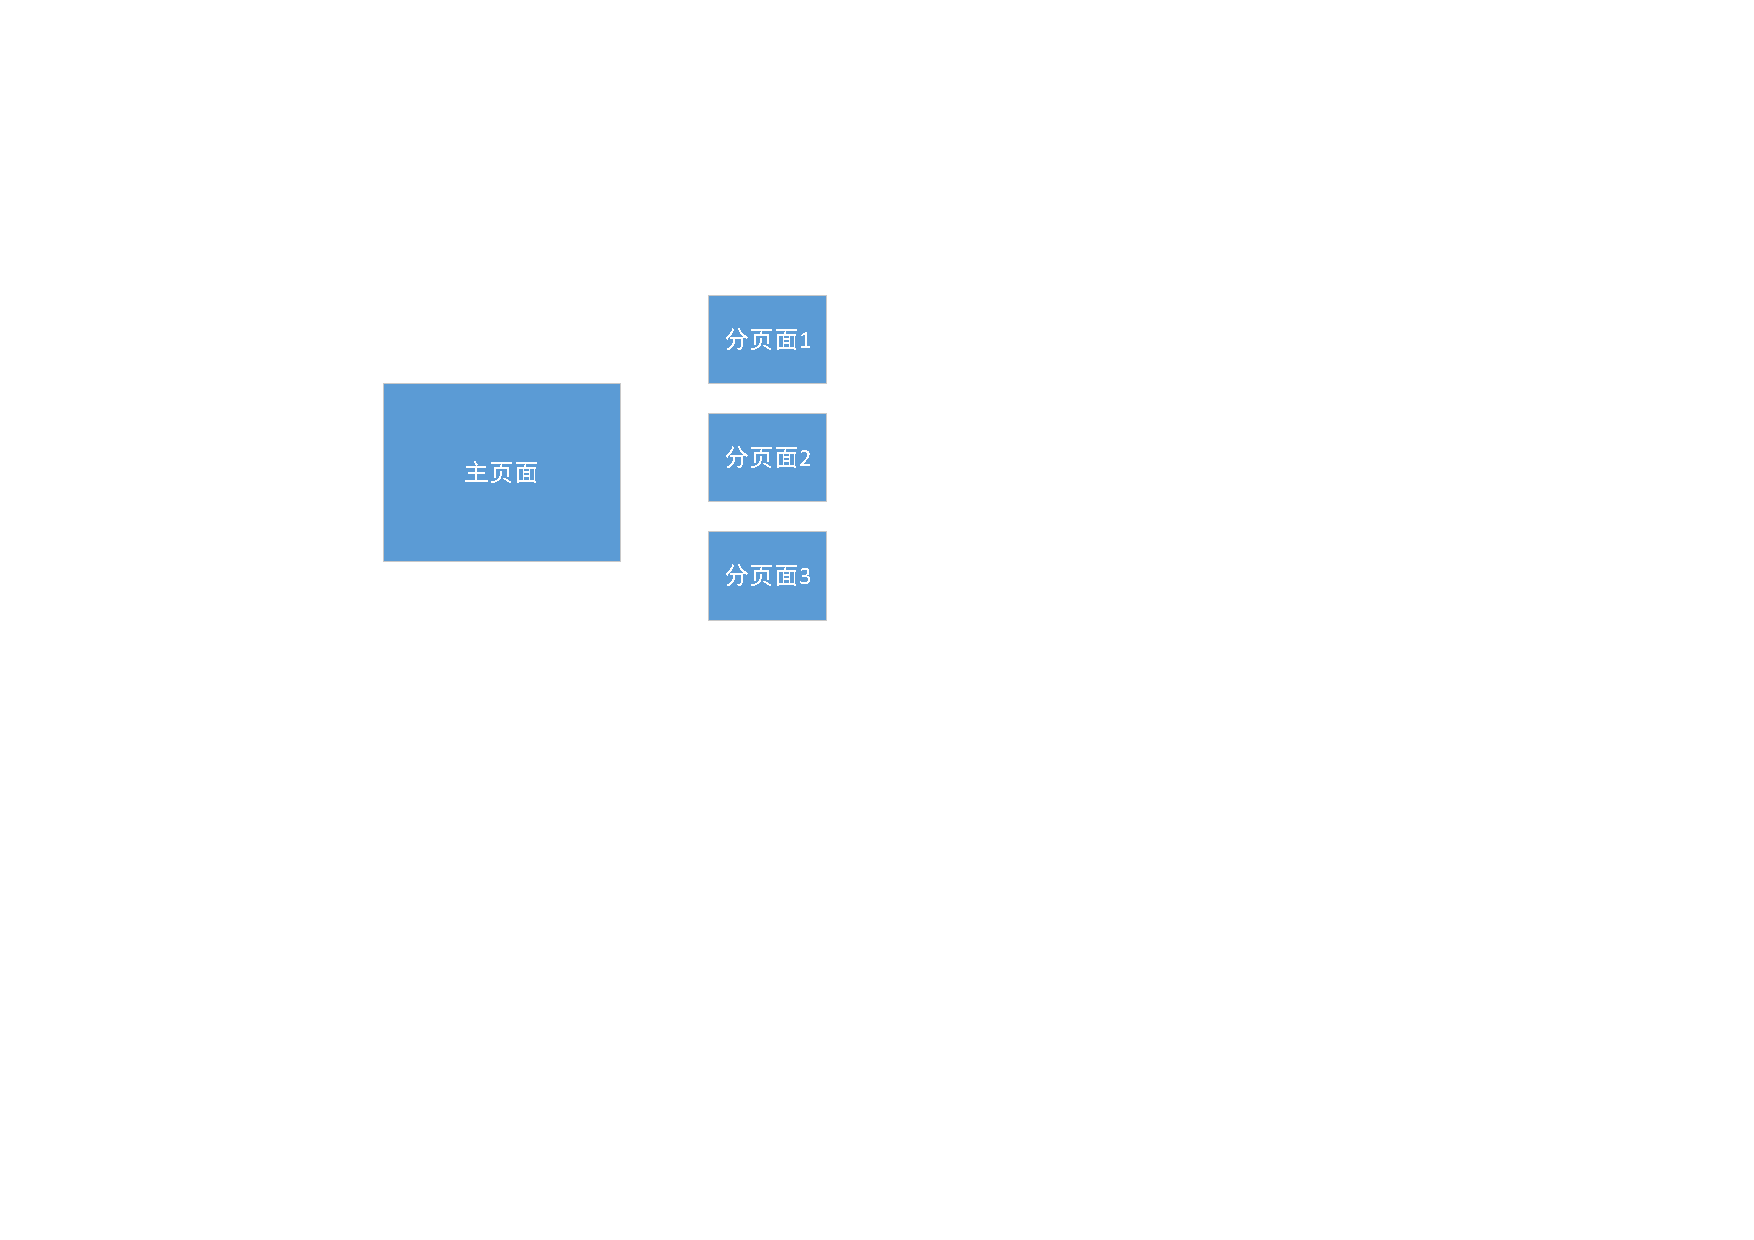
\includegraphics[scale=0.80]{images/1-1.pdf}
			\caption{网页整体框架举例}
			\label{fig1-1}
		\end{center}
	\end{figure}
	
	画图说明网页的整体框架，进行简要的文字描述等。画图说明网页的整体框架，进行简要的文字描述等。画图说明网页的整体框架，进行简要的文字描述等。画图说明网页的整体框架，进行简要的文字描述等。画图说明网页的整体框架，进行简要的文字描述等。画图说明网页的整体框架，进行简要的文字描述等。画图说明网页的整体框架，进行简要的文字描述等。
	
	\begin{figure}[htb]
		\begin{center}
			
\includegraphics[scale=0.60]{images/1-2.png}
			\caption{在visio里通过文件-打印，把visio图打印成pdf文件}
			\label{fig1-2}
		\end{center}
	\end{figure}
	
	画图说明网页的整体框架，进行简要的文字描述等。画图说明网页的整体框架，进行简要的文字描述等。画图说明网页的整体框架，进行简要的文字描述等。画图说明网页的整体框架，进行简要的文字描述等。画图说明网页的整体框架，进行简要的文字描述等。画图说明网页的整体框架，进行简要的文字描述等。画图说明网页的整体框架，进行简要的文字描述等。
	
	\begin{figure}[htb]
		\begin{center}
			
\includegraphics[scale=0.50]{images/1-3.png}
			\caption{用pdf阅览器的工具，对打印得到pdf图做适当的裁剪}
			\label{fig1-3}
		\end{center}
	\end{figure}
	
	画图说明网页的整体框架，进行简要的文字描述等。画图说明网页的整体框架，进行简要的文字描述等。画图说明网页的整体框架，进行简要的文字描述等。画图说明网页的整体框架，进行简要的文字描述等。画图说明网页的整体框架，进行简要的文字描述等。画图说明网页的整体框架，进行简要的文字描述等。画图说明网页的整体框架，进行简要的文字描述等。
	
	\newpage
	
	\section{主页设计}
	
	描述主页的结构，给出主页截图，描述主要设计思路等，请见图\ref{fig2-1}。描述主页的结构，给出主页截图，描述主要设计思路等。描述主页的结构，给出主页截图，描述主要设计思路等。描述主页的结构，给出主页截图，描述主要设计思路等。描述主页的结构，给出主页截图，描述主要设计思路等。描述主页的结构，给出主页截图，描述主要设计思路等。描述主页的结构，给出主页截图，描述主要设计思路等。
	
	\begin{figure}[htb]
		\begin{center}
			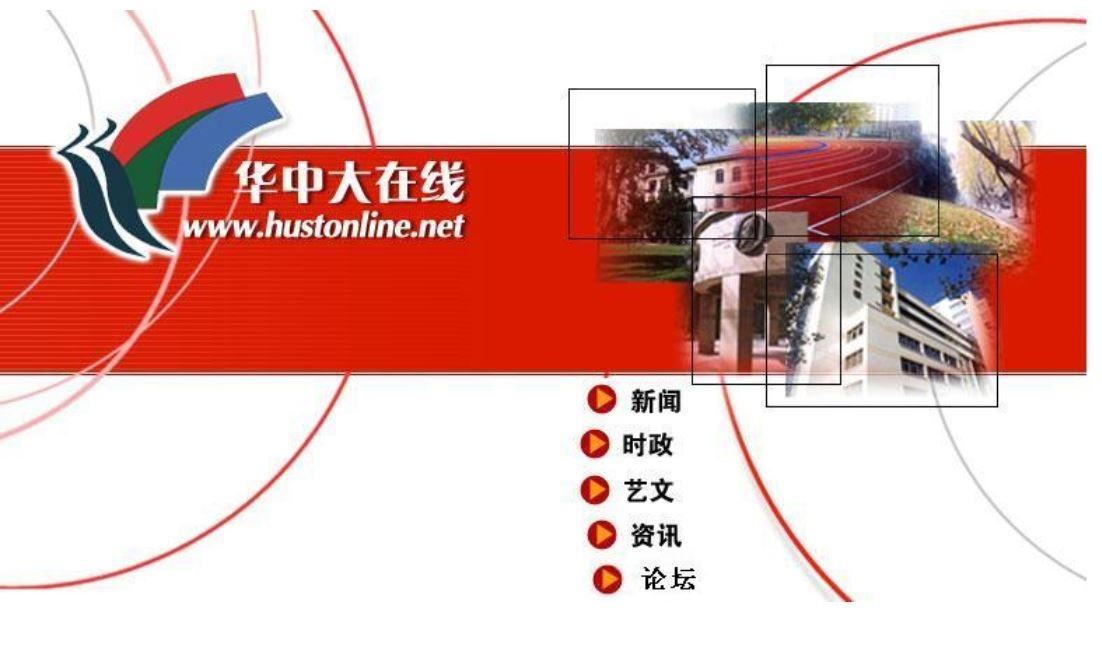
\includegraphics[scale=0.40]{images/2-1.jpg}
			\caption{主页举例}
			\label{fig2-1}
		\end{center}
	\end{figure}
	
	描述主页的结构，给出主页截图，描述主要设计思路等。描述主页的结构，给出主页截图，描述主要设计思路等。描述主页的结构，给出主页截图，描述主要设计思路等。描述主页的结构，给出主页截图，描述主要设计思路等。描述主页的结构，给出主页截图，描述主要设计思路等。描述主页的结构，给出主页截图，描述主要设计思路等。描述主页的结构，给出主页截图，描述主要设计思路等。
	
	描述主页的结构，给出主页截图，描述主要设计思路等。描述主页的结构，给出主页截图，描述主要设计思路等。描述主页的结构，给出主页截图，描述主要设计思路等。描述主页的结构，给出主页截图，描述主要设计思路等。描述主页的结构，给出主页截图，描述主要设计思路等。描述主页的结构，给出主页截图，描述主要设计思路等。描述主页的结构，给出主页截图，描述主要设计思路等。
	
	描述主页的结构，给出主页截图，描述主要设计思路等。描述主页的结构，给出主页截图，描述主要设计思路等。描述主页的结构，给出主页截图，描述主要设计思路等。描述主页的结构，给出主页截图，描述主要设计思路等。描述主页的结构，给出主页截图，描述主要设计思路等。描述主页的结构，给出主页截图，描述主要设计思路等。描述主页的结构，给出主页截图，描述主要设计思路等。
	
	描述主页的结构，给出主页截图，描述主要设计思路等。描述主页的结构，给出主页截图，描述主要设计思路等。描述主页的结构，给出主页截图，描述主要设计思路等。描述主页的结构，给出主页截图，描述主要设计思路等。描述主页的结构，给出主页截图，描述主要设计思路等。描述主页的结构，给出主页截图，描述主要设计思路等。描述主页的结构，给出主页截图。
	
	\newpage
	
	\section{分页面设计}
	
	给出分页面截图，描述主要设计思路等。给出分页面截图，描述主要设计思路等。给出分页面截图，描述主要设计思路等。给出分页面截图，描述主要设计思路等。
	
	\subsection{页面1 (每个页面以主要内容起标题名称即可）}
	
	给出分页面截图，描述主要设计思路等。给出分页面截图，描述主要设计思路等。给出分页面截图，描述主要设计思路等。给出分页面截图，描述主要设计思路等。给出分页面截图，描述主要设计思路等。给出分页面截图，描述主要设计思路等。给出分页面截图，描述主要设计思路等。给出分页面截图，描述主要设计思路等。给出分页面截图，描述主要设计思路等。给出分页面截图，描述主要设计思路等。给出分页面截图，描述主要设计思路等。给出分页面截图，描述主要设计思路等。给出分页面截图，描述主要设计思路等。
	
	如果实验报告中要用到算法伪代码，请参考算法\ref{alg:1}，也可以参考算法\ref{alg:2}。如果实验报告中要用到算法伪代码，请参考算法\ref{alg:1}，也可以参考算法\ref{alg:2}。如果实验报告中要用到算法伪代码，请参考算法\ref{alg:1}，也可以参考算法\ref{alg:2}。如果实验报告中要用到算法伪代码，请参考算法\ref{alg:1}，也可以参考算法\ref{alg:2}。
	
	\begin{shaded*}\begin{alg}{一个复杂算法}
			\label{alg:1}
			\begin{algorithmic}
				\Input Two numbers $a$ and $b$
				\Output The sum of $a$ and $b$
				\Procedure{A-Plus-B}{$a, b$}
				\If $a = 0$
				\State \Return $b$
				\EndIf
				\State $res \gets 0$
				\While{$b \neq 0$}
				\State Increase $res$ by $1$
				\State $b \gets b - 1$
				\EndWhile
				\State \Return $res$
				\EndProcedure
			\end{algorithmic}
	\end{alg}\end{shaded*}
	
	\subsection{页面2 (每个页面以主要内容起标题名称即可）}
	
	给出分页面截图，描述主要设计思路等。给出分页面截图，描述主要设计思路等。给出分页面截图，描述主要设计思路等。给出分页面截图，描述主要设计思路等。给出分页面截图，描述主要设计思路等。给出分页面截图，描述主要设计思路等。给出分页面截图，描述主要设计思路等。给出分页面截图，描述主要设计思路等。给出分页面截图，描述主要设计思路等。给出分页面截图，描述主要设计思路等。给出分页面截图，描述主要设计思路等。
	
	
	如果实验报告中要用到算法伪代码，请参考算法\ref{alg:1}，也可以参考算法\ref{alg:2}。如果实验报告中要用到算法伪代码，请参考算法\ref{alg:1}，也可以参考算法\ref{alg:2}。如果实验报告中要用到算法伪代码，请参考算法\ref{alg:1}，也可以参考算法\ref{alg:2}。如果实验报告中要用到算法伪代码，请参考算法\ref{alg:1}，华科计院不认同考算法\ref{alg:1}的格式，而认同具有三线表的算法\ref{alg:2}格式。
	
	\begin{algorithm}[h] 
		\caption{一个更复杂算法}
		\begin{algorithmic}[1]
			\State Initialization: $I_{xy}$, $z_{f}=Zeros(128, 128)$; 
			\For{$0\leq n \textless N$}
			\State $i=\lfloor x_n \rfloor+64$, $j=\lfloor y_n \rfloor + 64$
			\If{$z_n<0$ and $|z_n|>|z_{f}(i,j)|$};
			\State $z_{f}(i,j)=z_n$;
			\EndIf
			\State $I_{xy}(i,j)=z_{f}(i,j)$;
			\EndFor 
		\end{algorithmic}\label{alg:2}
	\end{algorithm}
	
	\subsection{页面3 (每个页面以主要内容起标题名称即可）}
	
	给出分页面截图，描述主要设计思路等。给出分页面截图，描述主要设计思路等。给出分页面截图，描述主要设计思路等。给出分页面截图，描述主要设计思路等。给出分页面截图，描述主要设计思路等。给出分页面截图，描述主要设计思路等。给出分页面截图，描述主要设计思路等。给出分页面截图，描述主要设计思路等。给出分页面截图，描述主要设计思路等。给出分页面截图，描述主要设计思路等。给出分页面截图，描述主要设计思路等。
	
	\subsection{页面4 (每个页面以主要内容起标题名称即可）}
	
	给出分页面截图，描述主要设计思路等。给出分页面截图，描述主要设计思路等。给出分页面截图，描述主要设计思路等。给出分页面截图，描述主要设计思路等。给出分页面截图，描述主要设计思路等。给出分页面截图，描述主要设计思路等。给出分页面截图，描述主要设计思路等。给出分页面截图，描述主要设计思路等。给出分页面截图，描述主要设计思路等。给出分页面截图，描述主要设计思路等。给出分页面截图，描述主要设计思路等。
	
	\newpage
	
	\section{网页设计小结}
	
	描述网页的设计和实现过程中遇到的问题及如何解决。描述网页的设计和实现过程中遇到的问题及如何解决。描述网页的设计和实现过程中遇到的问题及如何解决。描述网页的设计和实现过程中遇到的问题及如何解决。描述网页的设计和实现过程中遇到的问题及如何解决。描述网页的设计和实现过程中遇到的问题及如何解决。描述网页的设计和实现过程中遇到的问题及如何解决。描述网页的设计和实现过程中遇到的问题及如何解决。描述网页的设计和实现过程中遇到的问题及如何解决。
	
	描述网页的设计和实现过程中遇到的问题及如何解决。描述网页的设计和实现过程中遇到的问题及如何解决。描述网页的设计和实现过程中遇到的问题及如何解决。描述网页的设计和实现过程中遇到的问题及如何解决。描述网页的设计和实现过程中遇到的问题及如何解决。描述网页的设计和实现过程中遇到的问题及如何解决。描述网页的设计和实现过程中遇到的问题及如何解决。描述网页的设计和实现过程中遇到的问题及如何解决。描述网页的设计和实现过程中遇到的问题及如何解决。
	
	描述网页的设计和实现过程中遇到的问题及如何解决。描述网页的设计和实现过程中遇到的问题及如何解决。描述网页的设计和实现过程中遇到的问题及如何解决。描述网页的设计和实现过程中遇到的问题及如何解决。描述网页的设计和实现过程中遇到的问题及如何解决。描述网页的设计和实现过程中遇到的问题及如何解决。描述网页的设计和实现过程中遇到的问题及如何解决。描述网页的设计和实现过程中遇到的问题及如何解决。描述网页的设计和实现过程中遇到的问题及如何解决。
	
	描述网页的设计和实现过程中遇到的问题及如何解决。描述网页的设计和实现过程中遇到的问题及如何解决。描述网页的设计和实现过程中遇到的问题及如何解决。描述网页的设计和实现过程中遇到的问题及如何解决。描述网页的设计和实现过程中遇到的问题及如何解决。描述网页的设计和实现过程中遇到的问题及如何解决。描述网页的设计和实现过程中遇到的问题及如何解决。描述网页的设计和实现过程中遇到的问题及如何解决。描述网页的设计和实现过程中遇到的问题及如何解决。
	
	\newpage
	
	\section{课程的收获和建议}
	
	学习效率最好的方法，认真听讲，认真审题，认真模仿提供的例子。描述通过学习该专题，有何收获，有何建议，如某专题可适当减少讲授时间、某专题可适当增加讲授内容和时间等。描述通过学习该专题，有何收获，有何建议，如某专题可适当减少讲授时间、某专题可适当增加讲授内容和时间等。描述通过学习该专题，有何收获，有何建议，如某专题可适当减少讲授时间、某专题可适当增加讲授内容和时间等。描述通过学习该专题，有何收获，有何建议，如某专题可适当减少讲授时间、某专题可适当增加讲授内容和时间等。
	
	\subsection{计算机基础知识}
	
	描述通过学习计算机基础知识专题，有何收获，有何建议，如某专题可适当减少讲授时间、某专题可适当增加讲授内容和时间等。描述网页的设计和实现过程中遇到的问题及如何解决。描述网页的设计和实现过程中遇到的问题及如何解决。描述网页的设计和实现过程中遇到的问题及如何解决。描述网页的设计和实现过程中遇到的问题及如何解决。描述网页的设计和实现过程中遇到的问题及如何解决。描述网页的设计和实现过程中遇到的问题及如何解决。描述网页的设计和实现过程中遇到的问题及如何解决。描述网页的设计和实现过程中遇到的问题及如何解决。明年要讲一下什么是资源管理器，怎么新建文件夹与文件。怎么装正版的软件，特别是winrar。还要提前提醒大家不要装任何电脑管家。
	
	\subsection{文档撰写工具LaTeX}
	
	描述通过学习文档撰写工具LaTeX专题，有何收获，有何建议，如某专题可适当减少讲授时间、某专题可适当增加讲授内容和时间等。描述通过学习文档撰写工具LaTeX专题，有何收获，有何建议，如某专题可适当减少讲授时间、某专题可适当增加讲授内容和时间等。插入参考文献、表格、公式、图是LaTeX最基本的操作，考核题目不能再简单了。如何插入算法，需要大家对照提供的例子去模仿。还记得部分同学看到cmd窗口里``请按任意键继续''后手足无措的样子!
	
	\subsection{编程工具Python}
	
	Python讲都是基础知识，如果讲慢了，基础就讲不完了，讲快了部分同学们又跟不上，这个矛盾怎么解决？描述通过学习编程工具Python专题，有何收获，有何建议，如某专题可适当减少讲授时间、某专题可适当增加讲授内容和时间等。描述通过学习编程工具Python专题，有何收获，有何建议，如某专题可适当减少讲授时间、某专题可适当增加讲授内容和时间等。装环境、配解释器、矩阵运算、图像操作等是实际开发的利器，希望大家巩固掌握。Python语法就那么一点，基础入门并不难的。编程习惯很重要，胜过语法本身，部分同学还没有改掉用绝对路径的毛病！部分同学试图实现跨文件夹的import！出问题不可怕，可怕的是不按照规范来施行！
	
	\subsection{图像设计软件Photoshop}
	
	流程图一定要画的规范。Visio是画流程图的好帮手，记得在视图里勾上grid。描述通过学习Photoshop与Visio专题，有何收获，有何建议，如某专题可适当减少讲授时间、某专题可适当增加讲授内容和时间等。描述通过学习计算机基础知识专题，有何收获，有何建议，如某专题可适当减少讲授时间、某专题可适当增加讲授内容和时间等。同学们可以再这里贴上你骄傲的作品。课程内容相对较好，每个实践例子老师表演了2到3遍。部分进校时的小白同学通过课下温习，掌握的非常好。
	
	\subsection{版本管理软件Git}
	
	描述通过学习图像设计软件Git专题，有何收获，有何建议，如某专题可适当减少讲授时间、某专题可适当增加讲授内容和时间等。描述通过学习图像设计软件Photoshop专题，有何收获，有何建议，如某专题可适当减少讲授时间、某专题可适当增加讲授内容和时间等。先送给大家一千万：千万不能用中文注册github或者gitee的账号！add remote添加远程仓库是最容易出问题的地方，错误的种类千千万，操作正确的道路就一条。再送每人两千万：千万不要添加错了远程仓库的地址，不千万要搞混远程仓库地址中的用户名及其与之关联的字段。
	
	\subsection{网页制作Dreamweaver}
	
	描述通过学习网页制作Dreamweaver专题，有何收获，有何建议，如某专题可适当减少讲授时间、某专题可适当增加讲授内容和时间等。描述通过学习网页制作Dreamweaver专题，有何收获，有何建议，如某专题可适当减少讲授时间、某专题可适当增加讲授内容和时间等。还记得老师送的两千万吗？绝对路径千万不可取，资源路径千万要放在工作区！
	
	
	\nocite{*} %% 作用是不对文献进行引用，但可以生成文献列表
	
	\bibliographystyle{Experimental_Report}
	\bibliography{Experimental_Report}
	\setcounter{secnumdepth}{0}
	\appendix
	
	\section{附录A 功能模块一实现的主要源程序}
	
	\noindent
	/* Linear Table On Sequence Structure */\\
	\#include <stdio.h>\\
	\#include <malloc.h>\\
	\#include <stdlib.h>\\
	
	\noindent
	/*---------page 10 on textbook ---------*/\\
	\#define TRUE 1\\
	\#define FALSE 0\\
	\#define OK 1\\
	\#define ERROR 0\\
	\#define INFEASTABLE -1\\
	\#define OVERFLOW -2\\
	\newpage
	\section{附录B 功能模块二实现的主要源程序}
	\newpage
	\section{附录C 功能模块三实现的主要源程序}
	\newpage
	\section{附录D 功能模块四实现的主要源程序}
	
\end{document}